\section{Algorithms for calculation of the Green function}

\begin{framenologo}
  \frametitle{Algorithms for calculation of the Green function}
  \tableofcontents[currentsection]
\end{framenologo}


\subsection{Problems in NEGF}

\begin{framenologo}
  \frametitle{Algorithms for calculation of the Green function}
  \framesubtitle{Equations again --- and problems herein}
  
  \begin{block}{NEGF equations}
    \vskip -2ex
    \begin{align*}
      \DM & =\frac1{2\pi}
      \iint_\BZ\dEBZ\cd \kk \dd\E\, \sum_\idxE\G_\kk(\E)\Scat_{\idxE,\kk}(\E)\G_\kk^\dagger(\E) n_{F,\idxE}(\E)
      \eikr
      \\
      \G_\kk(\E)&=\big[(\E+\im\eta)\SO_\kk - \HH_\kk - \sum_\idxE\SE_{\idxE,\kk}(\E-\mu_\idxE)\big]^{-1}
      \\
      \Scat_{\idxE,\kk}(\E) &=\im\big(\SE_{\idxE,\kk}(\E-\mu_\idxE)-\SE^\dagger_{\idxE,\kk}(\E-\mu_\idxE)\big)
    \end{align*}
  \end{block}

  \begin{block}{Problems}
    \begin{itemize}
      \item Matrix inversion to calculate the Green function
      \item Green function dimension determined from \# of orbitals ($N$)
      \item Elements in matrix scales $N^2$, inversion has complexity $\mathcal O(N^3)$
    \end{itemize}
  \end{block}

  \begin{block}<2->{Solvable problems}
    \begin{itemize}
      \item Only a subset of the Green function is needed (Hamiltonian sparsity pattern)
      \item Different algorithms for \emph{selective} inversion exists, (BTD, MUMPS,
      PEXSI, \dots)
    \end{itemize}
  \end{block}

\end{framenologo}


\begin{frame}
  \frametitle{Algorithms for calculation of the Green function}
  \framesubtitle{Implemented algorithms}

  \footnotesize
  \begin{block}{\small LAPACK, full matrices}

    \begin{description}
      \item[-] Slow
      \item[-] Memory hungry
      \item[+] Very easy to implement
    \end{description}

  \end{block}

  \begin{block}{\small MUMPS, sparse matrices}

    \begin{description}
      \item[-] Serial and slow
      \item[-] Memory hungry (compared to BTD)
      \item[-] Slow for wide electrodes due to dense Green function requirement
      \item[+] Relatively easy to implement, special MUMPS memory layout (which is nicely documented)
      \item[+] May be extended to parallel execution
      \item[+] Ideal for tight-binding matrices due to extreme sparsity
    \end{description}

  \end{block}

  \begin{block}{\small Block-Tri-Diagonal, block tri diagonal matrices}

    \begin{description}
      \item[-] Limited by width of electrodes
      \item[-] Hard to implement (only triple product)
      \item[+] Fast
      \item[+] Memory efficient for narrow electrodes
    \end{description}

  \end{block}

\end{frame}



\subsection{Block Tri Diagonal inversion (BTD)}

\begin{frame}
  \frametitle{Block tri-diagonal inversion}

  \begin{itemize}
    %
    \item
    Reducing the inversion algorithm to take advantage of the intrinsic block tri-diagonality of
    the sparsity pattern

    \begin{columns}[c]
      
      \column{.5\textwidth}
      
      \begin{equation*}
        \mathbf G^{-1}=
        \begin{pmatrix}
          \bm A_1 & \bm C_2 & 0 & &\cdots \\
          \bm B_1 & \bm A_2 & \bm C_3 & 0& \cdots \\
          0 & \bm B_2 &\ddots & \ddots \\
          & 0  & \ddots & & \bm C_p \\
          \vdots & \vdots  &   & \bm B_{p-1} & \bm A_p\\
        \end{pmatrix}
      \end{equation*}

      \column{.5\textwidth}

      \begin{align*}
        \widetilde{\mathbf Y}_n&=\left[\mathbf A_{n-1}-\mathbf Y_{n-1}\right]^{-1}
        \mathbf C_n %
        & & \mathbf Y_1=0
        \\
        \mathbf Y_n&=\mathbf B_{n-1}\widetilde{\mathbf Y}_n
        \\
        \widetilde{\mathbf X}_n & =\left[\mathbf A_{n+1}-\mathbf X_{n+1}\right]^{-1}
        \mathbf B_n %
        & & \mathbf X_p=0
        \\
        \mathbf X_n & =\mathbf C_{n+1}\widetilde{\mathbf X}_n
      \end{align*}

    \end{columns}

    \begin{align*}
      \left.
        \begin{aligned}
          \G_{n,n}&=\left[\mathbf A_n-\mathbf X_n-\mathbf Y_n\right]^{-1},
          \\
          \G_{m-1,n}&%=-\left[\mathbf A_m-\mathbf Y_m\right]^{-1}\mathbf C_{m+1} \G_{m+1,n}
          =
          -\widetilde{\mathbf Y}_{m} \G_{m,n}\quad\text{ for }m\le n,
          \\
          \G_{m+1,n}&%=-\left[\mathbf A_m-\mathbf X_m\right]^{-1}\mathbf B_{m-1} \G_{m-1,n}
          =
          -\widetilde{\mathbf X}_{m} \G_{m,n}\quad\text{ for }m\ge n,
        \end{aligned}\qquad
      \right\}\quad\G = 
      \begin{aligned}
        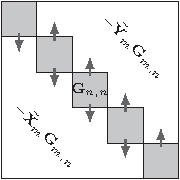
\includegraphics{G_recursion}
      \end{aligned}
    \end{align*}
    
    \item Note that this is a \emph{general} algorithm, it does not require Hermiticity 
    
  \end{itemize}
  
  \vskip 2em

  \doicite{Papior \etal: \doi{10.1016/j.cpc.2016.09.022}}

\end{frame}



\subsection{Pivoting for BTD}


\begin{frame}[fragile]
  \frametitle{Enforcing BTD --- going quasi 1D}
  \framesubtitle{Pivoting matrix elements, order from dis-order}

  \begin{columns}
    \begin{column}{.45\linewidth}
      \begin{itemize}
        \item 2,400 atoms
        \item 21,600 orbitals
      \end{itemize}
      \incg[width=1\linewidth]{dev2}
      
      \begin{equation*}
        \scriptsize
        \text{\huge \only<1>{?}}\quad
        \begin{pmatrix}
          \mathbf A_1 & \mathbf C_2 & 0 & \cdots & \\
          \mathbf B_1 & \mathbf A_2 & \mathbf C_3 & 0& \cdots \\
          0 & \mathbf B_2 &\ddots & \ddots & 0 \\
          \vdots & 0  & \ddots &  \ddots & \mathbf C_p \\
          & \vdots  & 0  & \mathbf B_{p-1} & \mathbf A_p\\
        \end{pmatrix}\quad\text{\huge \only<1>{?}}
      \end{equation*}
      
    \end{column}
    \begin{column}<2->{.55\linewidth}
      \begin{itemize}
        \item White $=0$
        \item Black $\neq0$
      \end{itemize}
      \begin{center}
        \href{run:fig/pivoting.mp4}{%
            \begin{tikzpicture}%
              \only<2>{
                  \node[inner sep=0pt,outer sep=0pt,draw,thick] (A) {%
                      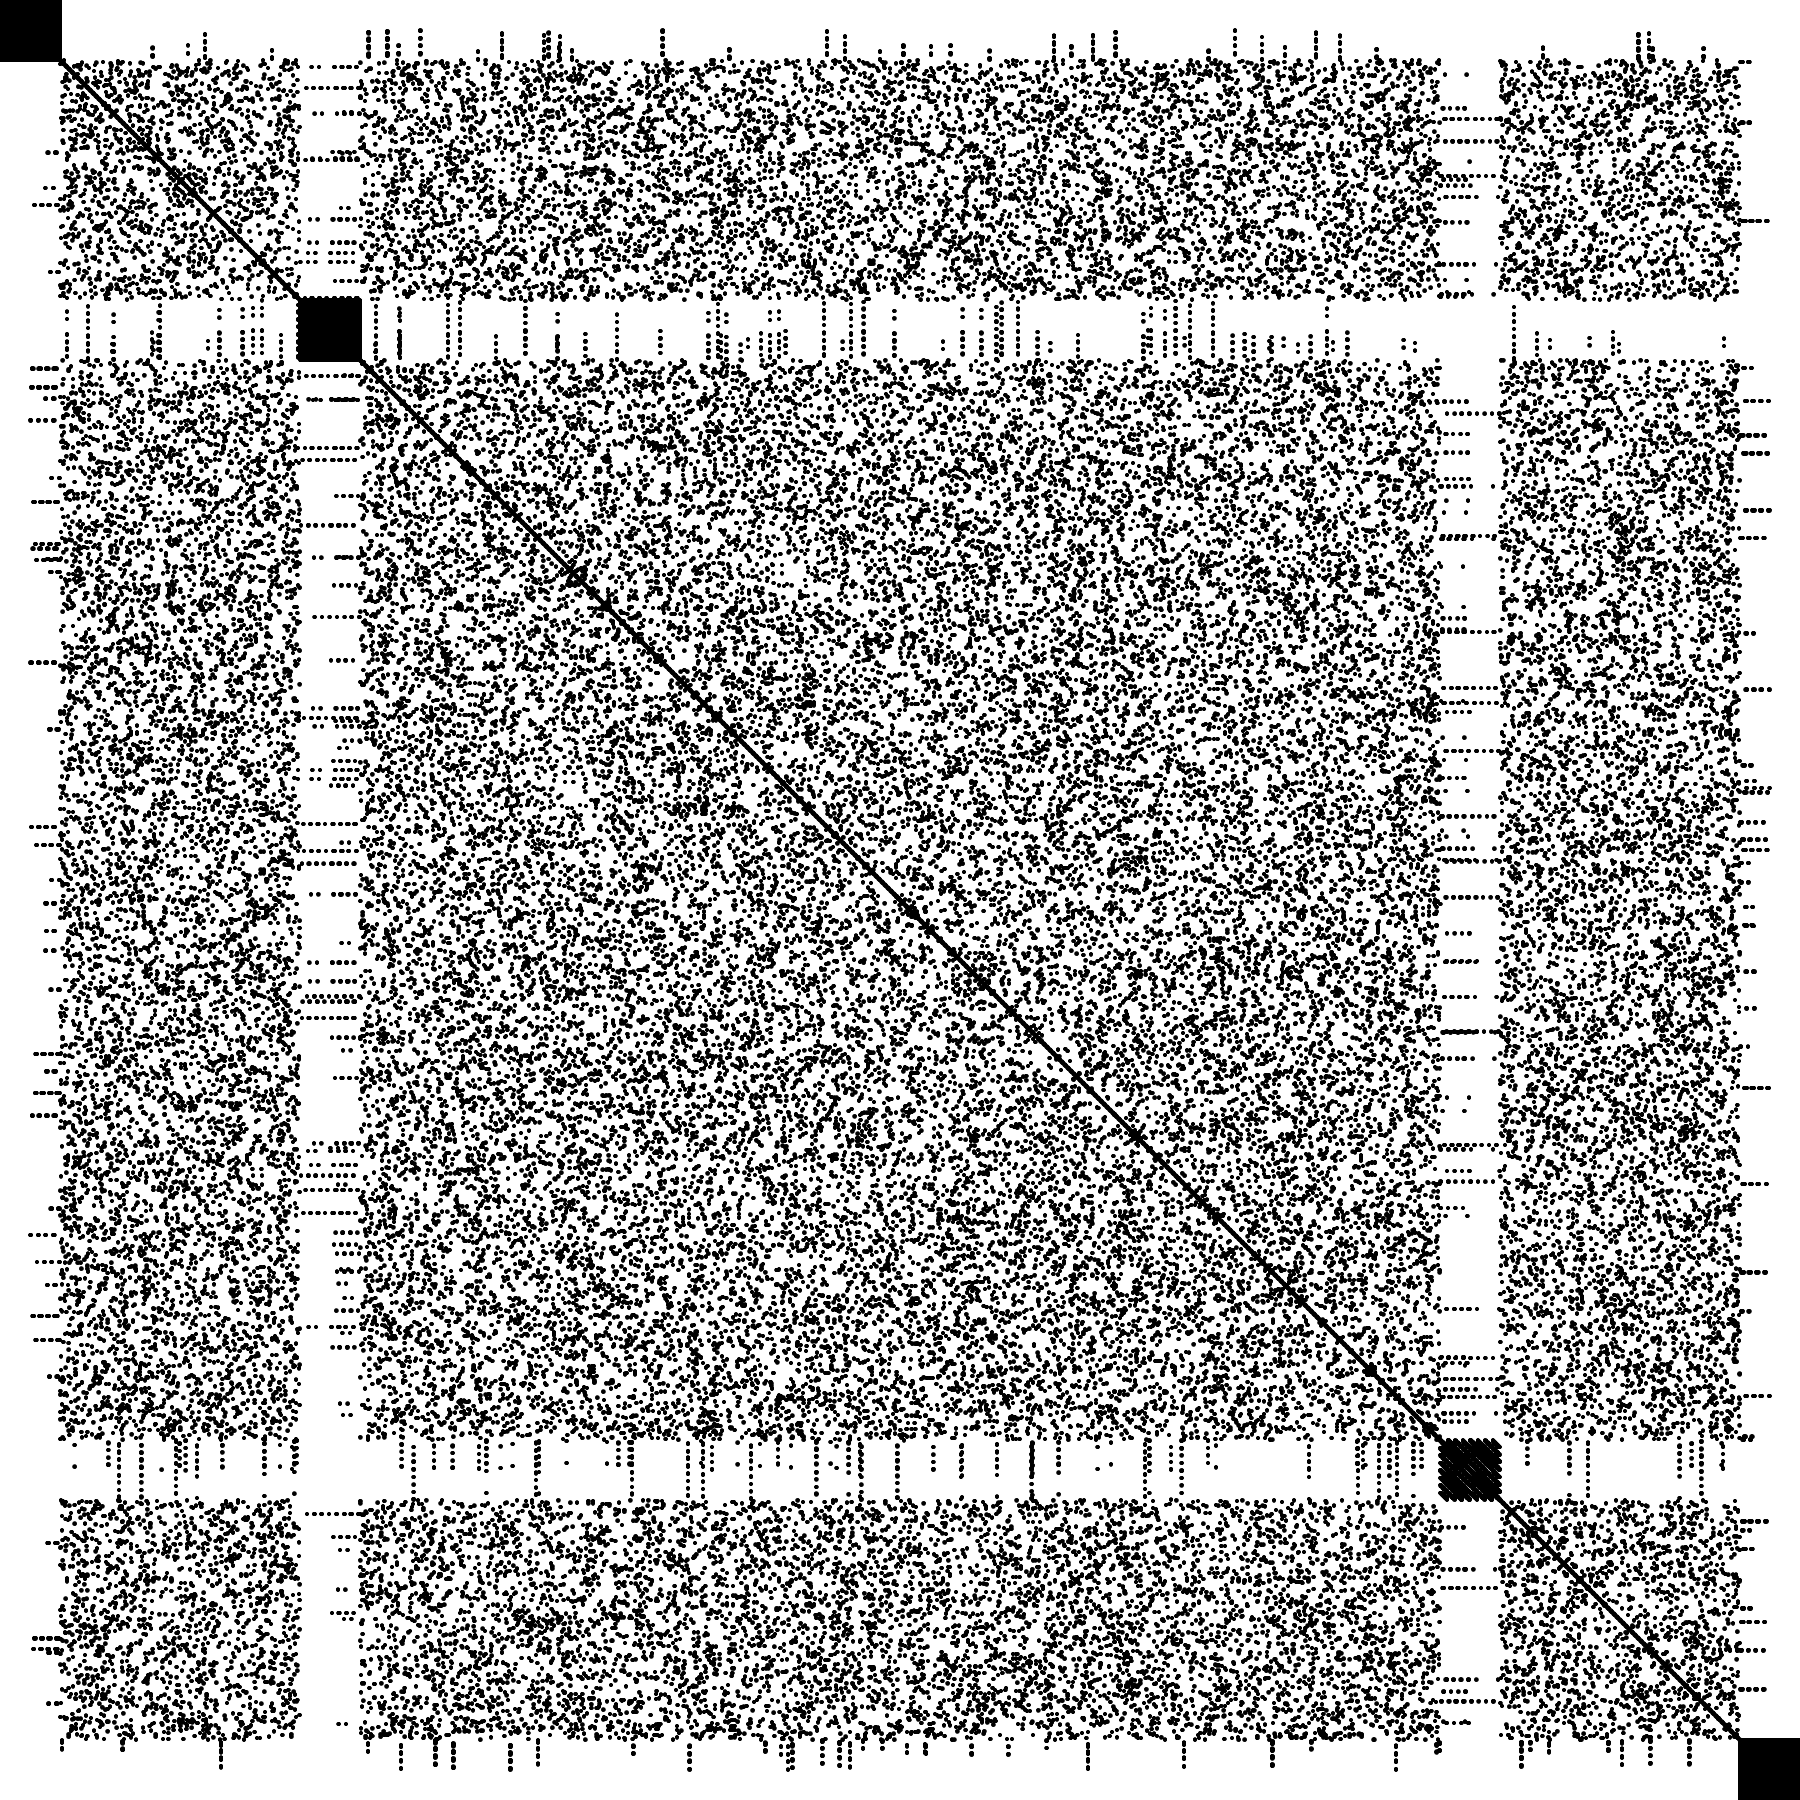
\includegraphics[height=.5\textheight]{atom+el-3_ani_0}};
                  \draw[->] ($(A.west)!.97!(A.north west)-(.5,0)$) node[left,green] {Elec-1} -- ++(.4,0);
                  \draw[->] ($(A.west)!.64!(A.north west)-(.5,0)$) node[left,red] {Elec-2} -- ++(.4,0);
                  \draw[->] ($(A.west)!.64!(A.south west)-(.5,0)$) node[left,blue] {Elec-3} --
                  ++(.4,0);
                  \draw[->] ($(A.west)!.97!(A.south west)-(.5,0)$) node[left,purple] {Elec-4} -- ++(.4,0);
              }
              \only<3>{
                  \node[inner sep=0pt,outer sep=0pt,draw,thick] (A) {%
                      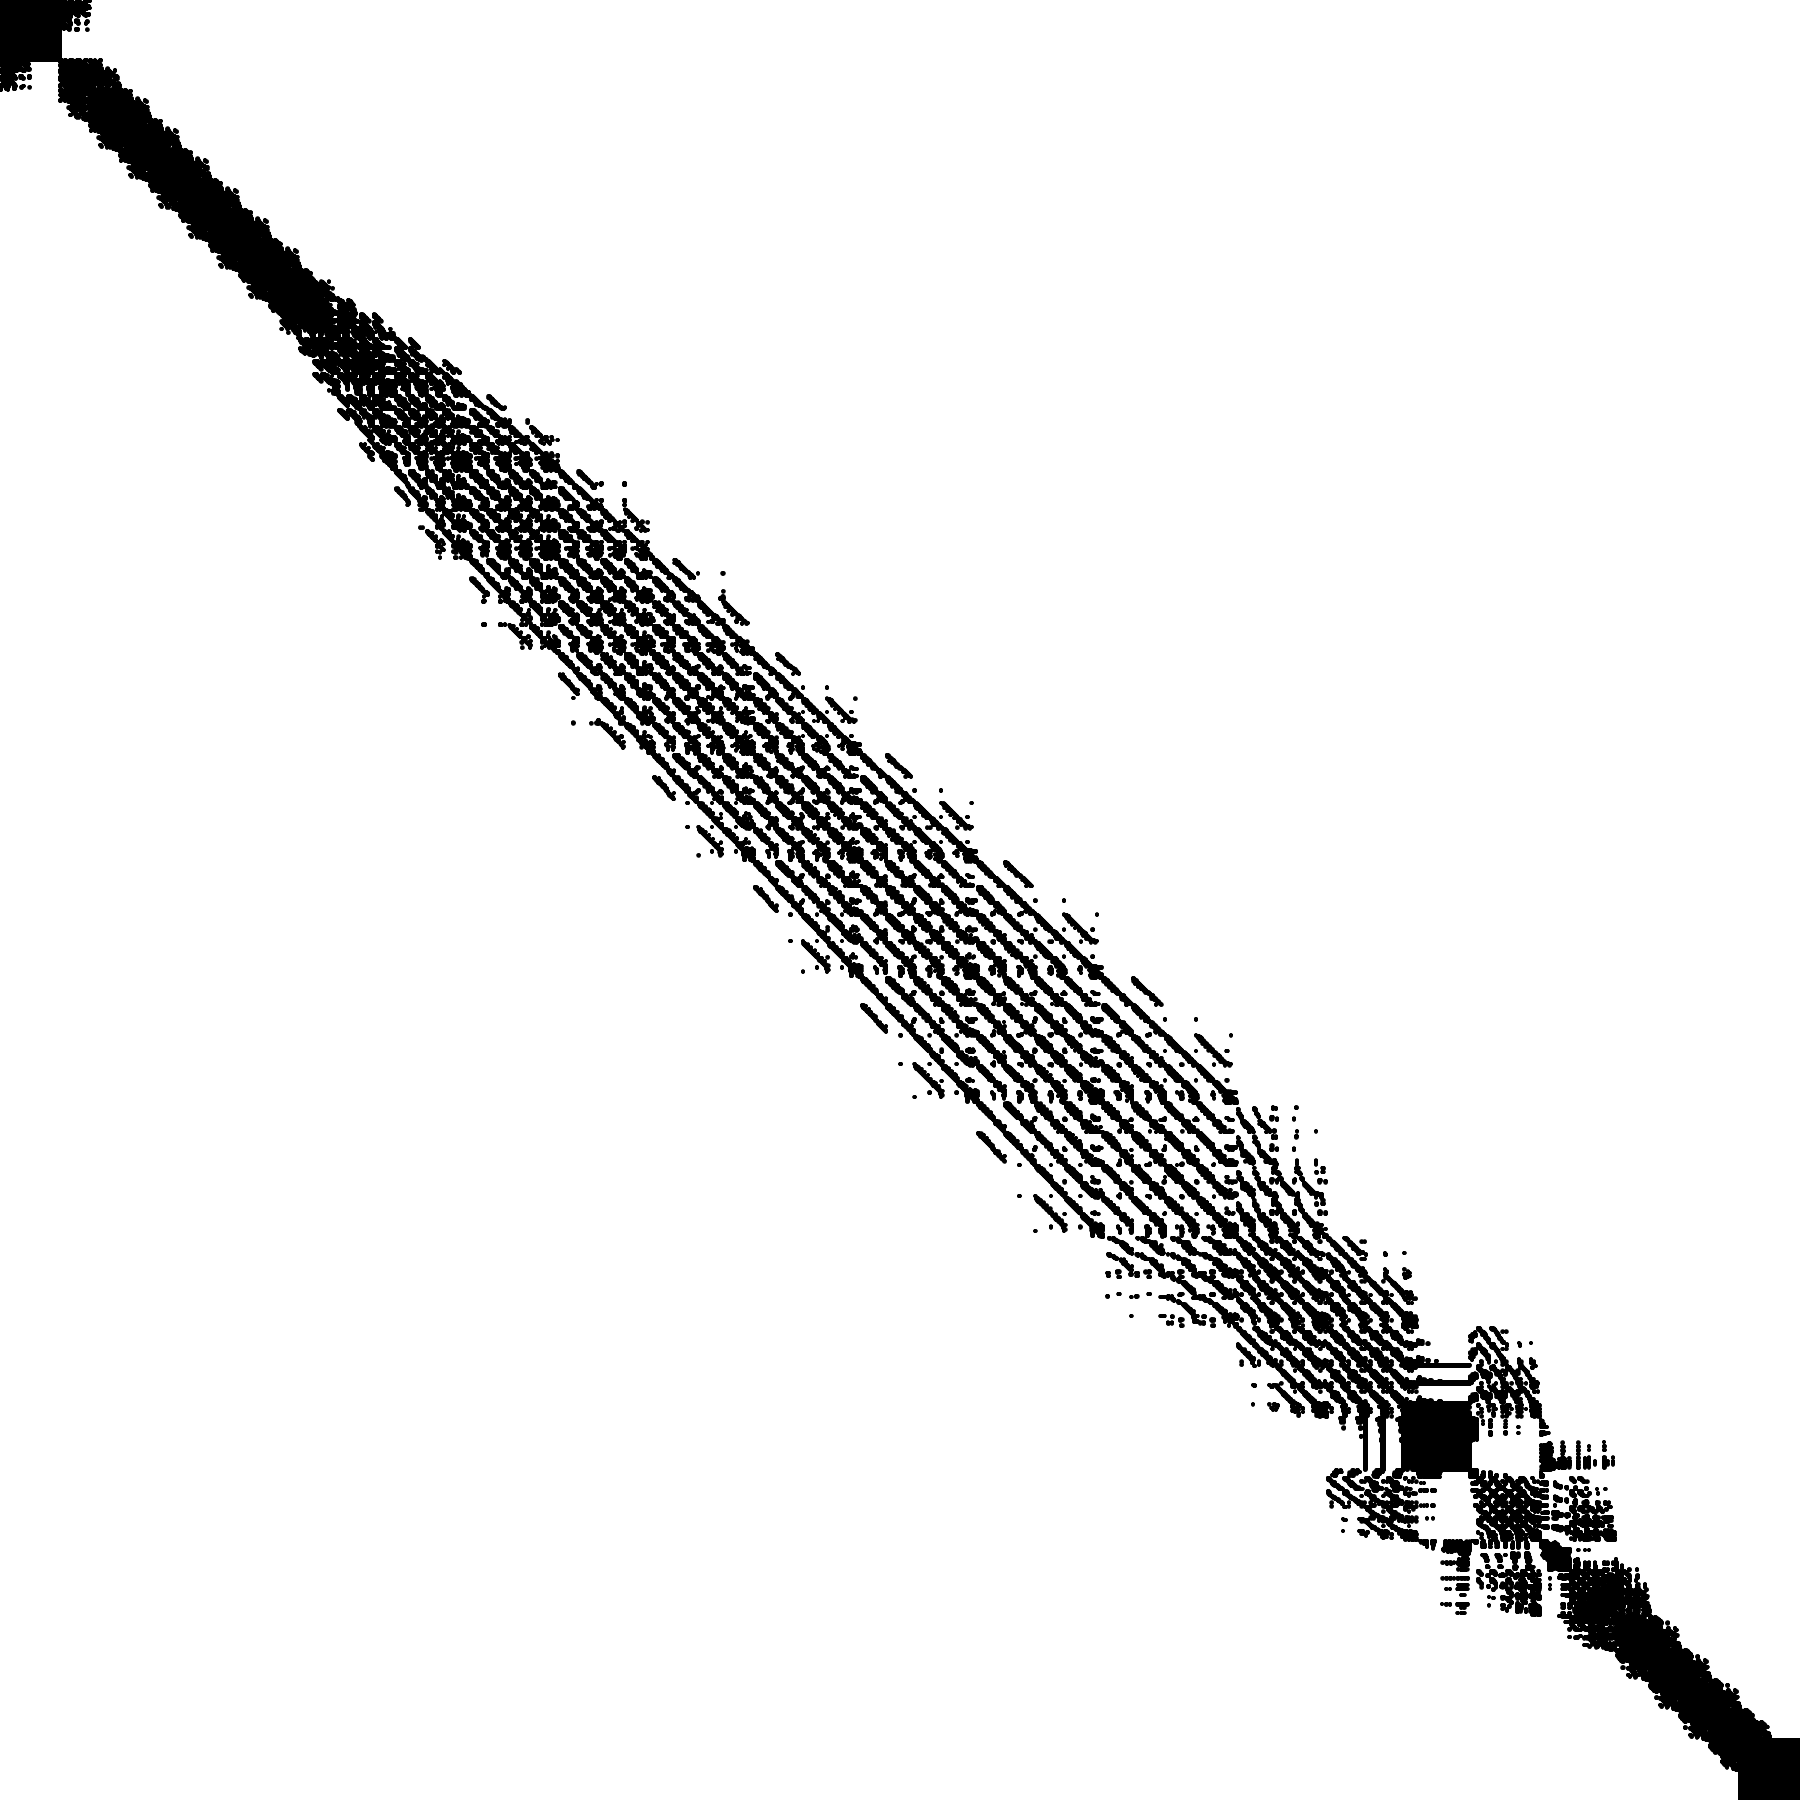
\includegraphics[height=.5\textheight]{atom+el-3_ani_21483}};
                  \draw[->] ($(A.west)!.97!(A.north west)-(.5,0)$) node[left,blue!80!black] {Elec-3} -- ++(.4,0);
                  \draw[->] ($(A.west)!.64!(A.north west)-(.5,0)$) node[left,purple!80!black] {Elec-4} -- ++(.4,0);
                  \draw[->] ($(A.west)!.64!(A.south west)-(.5,0)$) node[left,red!80!black] {Elec-2} --
                  ++(.4,0);
                  \draw[->] ($(A.west)!.97!(A.south west)-(.5,0)$) node[left,green!80!black] {Elec-1} -- ++(.4,0);
              }
            \end{tikzpicture}%
        }
      \end{center}
    \end{column}
  \end{columns}

\end{frame}


\def\tmpig#1{\fbox{\incg[width=.3\linewidth]{#1}}}
\begin{framenologo}
  \setlength\fboxsep{0pt}
  \frametitle{Other pivoting schemes}
  \framesubtitle{An ongoing investigation in Finite Element Methods}

  \begin{tabular}{ccc}
    Elec-1 & Elec-2 & Elec-3
    \\
    \tmpig{atom+el-1} & \tmpig{atom+el-2} & \tmpig{atom+el-3}
    \\
    reverse Cuthill-McKee & Gibbs-Poole-Stockmeyer & Gen. Gibbs-Poole-Stockmeyer
    \\
    \tmpig{atom+rev-CM} & \tmpig{atom+GPS} & \tmpig{atom+GGPS}
  \end{tabular}

  \begin{tikzpicture}[remember picture,overlay]
    \node[opacity=.8,anchor=north east] at (current page.north east) 
    {\incg[width=5cm]{dev2}};

    \node[opacity=.8,scale=.5,anchor=south west,outer sep=2*\framesep] at ($(current page.south west)+(0,.3)$)
    {$\begin{pmatrix}
          \mathbf A_1 & \mathbf C_2 & 0 & \cdots & \\
          \mathbf B_1 & \mathbf A_2 & \mathbf C_3 & 0& \cdots \\
          0 & \mathbf B_2 &\ddots & \ddots & 0 \\
          \vdots & 0  & \ddots &  \ddots & \mathbf C_p \\
          & \vdots  & 0  & \mathbf B_{p-1} & \mathbf A_p\\
        \end{pmatrix}$
    };

  \end{tikzpicture}

  \doicite{{CutHill: \doi{10.1145/800195.805928}, GPS: SIAM Numerical Analysis - 1976},
      GGPS: Progress In Electromagnetics Research - 2009}

\end{framenologo}



\algnewcommand\algorithmicto{\textbf{to}}
\algrenewtext{For}[2]%
{\algorithmicfor\ #1 \algorithmicto\ #2 \algorithmicdo}



\subsection{Efficient calculation of the spectral function}

\begin{frame}
  \frametitle{Efficient calculation of the spectral function}

  \begin{itemize}[<+->]
    \item Using the full matrix $\G_\kk$ and then the product $\G_\kk\Scat\G_\kk^\dagger$
    \begin{equation*}
      \Full \;\; \Left \;\; \Full ^\dagger = \Full
    \end{equation*}
    \item However, only the black elements are required for the MM
    \begin{equation*}
      \FullLeft \;\; \Left \;\; \FullLeft ^\dagger = \Full\;,
    \end{equation*}
    which means we need not calculate the full $\G_\kk$

    \begin{equation*}
      \Spec_{\idxE} =
      \begin{aligned}
        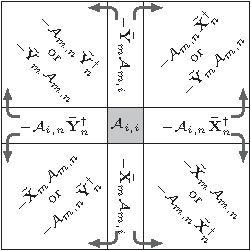
\includegraphics{A_recursion}
      \end{aligned}.
    \end{equation*}

  \end{itemize}

  \vskip 2em

  \doicite{Papior \etal: \doi{10.1016/j.cpc.2016.09.022}}

\end{frame}



\subsection{Method comparisons}


\begin{frame}
  \frametitle{Method comparisons}
  \framesubtitle{Performance}

  \begin{itemize}
    \item Graphene of varying length (BTD ideal)
    \item Tested with, MUMPS, LAPACK and BTD
  \end{itemize}

  \begin{center}
    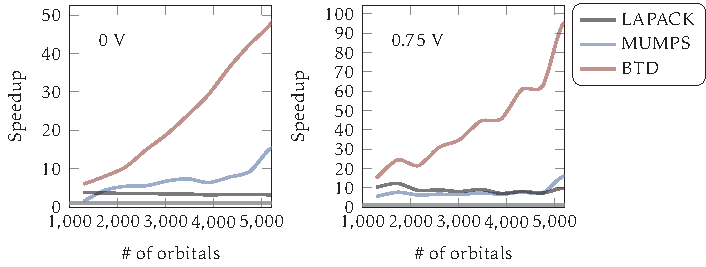
\includegraphics[height=.3\textheight]{perf_method_old}
    
    \uncover<2->{%
    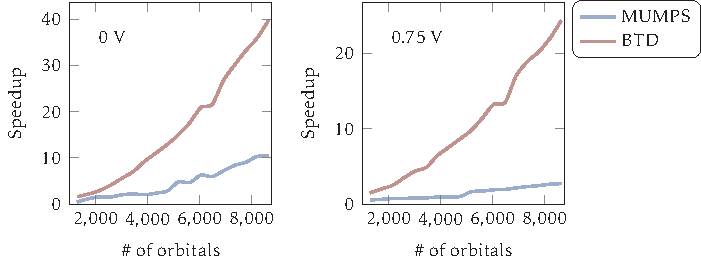
\includegraphics[height=.3\textheight]{perf_method_new}}
  \end{center}

  \uncover<3->{
      \begin{center}
        Typically BTD is the fastest method!
      \end{center}
  }

  \doicite{Papior \etal: \doi{10.1016/j.cpc.2016.09.022}}

\end{frame}


\def\setup#1#2{
    \def\bw{#1}
    \def\bh{#2}
    \pgfmathparse{\bw * 2}
    \edef\bwtwo{\pgfmathresult}
    \pgfmathparse{\bw * 4}
    \edef\bwfour{\pgfmathresult}
    \pgfmathparse{\bw * 5}
    \edef\bwfive{\pgfmathresult}
    \pgfmathparse{\bw * 8}
    \edef\bweight{\pgfmathresult}
}

\subsection{Transmission algorithm}


\begin{frame}[fragile]
  \frametitle{Calculating the Green function, slightly differently}
  
  \begin{itemize}
    \item Reduce Green function calculation to region of interest ($D$)

    \item Algorithms determined from user-requested quantities

  \end{itemize}

  \vskip 4em

  \begin{itemize}
    \item Algorithm:
  \end{itemize}
  \begin{center}
    \incg[]{tbt-algorithm}
  \end{center}

  \uncover<2->{
      \begin{tikzpicture}[remember picture,overlay]
        \node at ($(current page.center)+(2.5,1.6)$) {%
            \incg[width=.7\linewidth]{inv-block3}%
        };
      \end{tikzpicture}
  }

  \doicite{Papior \etal: \doi{10.1016/j.cpc.2016.09.022}}

\end{frame}





%%% Local Variables:
%%% mode: latex
%%% TeX-master: "talk"
%%% End:
